\chapter{Développement Android}
\section{Les différents composants d'Android}
Google met à disposition des développeurs un kit de développement (SDK) complet et une API (interface de développement) très bien documenté pour développer des applications Android. Nous allons voir dans cette partie les bases du développement sous Android et l'architecture du projet.
\subsection{Les activités}
Les applications Android fonctionne avec ce que l'on appelle des activités (classe \verb!Activity!) et des fragments (\verb!Fragment!).
Une Activité représente la totalité du contenu affiché à l'écran. Pour créer une nouvelle activité on créer donc une classe java qui va étendre la classe \verb!Activity!. Les activités ne peuvent échanger entre elles que des paramètres de types simples (booléens, chaines de caractères, entiers...). Pour pouvoir afficher le contenu souhaité dans une nouvelle activité nous passons donc à l'activité essentiellement les identifiants des objets à traiter sous forme d'entier.\bigskip

Le diagramme ci-dessous explique le cycle de vie d'une activité avec les différentes méthodes appelées à chaque événement. Ce diagramme nous a été très utile pour comprendre la mécanique de transition entre les activités. En effet lorsque l'on instancie une nouvelle activité, la précédente se met dans une pile d'activités et continue à consommer des ressources du système. Il est donc plus que nécessaire de connaître le traitement à effectuer en fonction de chaque cas.

\begin{img}
  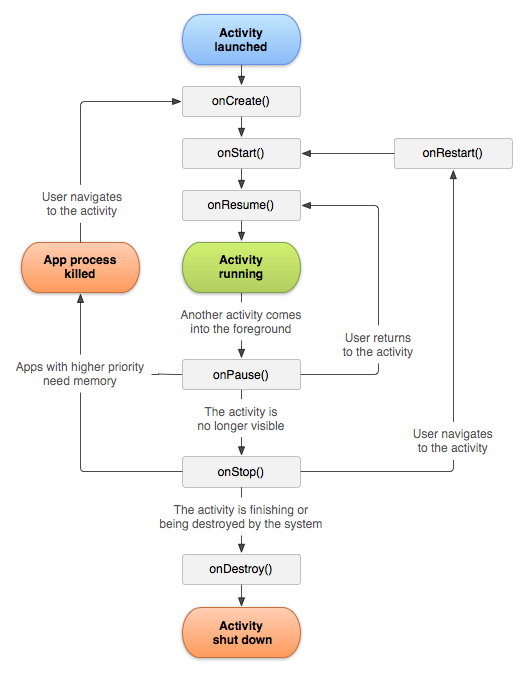
\includegraphics[scale=0.5]{img/cycle.png}
  \caption{Cycle de vie d'une Activity}
\end{img}

Les méthodes les plus importantes dans notre développement sont:\bigskip
 \begin{itemize}
 	\item \verb!onCreate()! lancé au démarrage de l'activité. C'est ici que l'ont peux récupérer les valeurs passées en paramètre de l'activité et ainsi instancier les objets nécessaires.
 	\item \verb!onRestart()! lancé lorsque l'utilisateur utilise la touche précédent de son smartphone. L'activité dans la pile d'activités déjà instancié une première fois doit alors vérifier les données à mettre à jour pour actualiser l'affichage.
 \end{itemize}

\subsection{Les fragments}
Les fragments (classe \verb!Fragment!) sont des sous-activités qui peuvent être intégrés dans une activité (par exemple une liste ou une boite de dialogue). Ils possèdent le même cycle de vie que les activités à l'exception de deux méthodes supplémentaires:\bigskip
 
\begin{itemize}
 	\item \verb!onAttach()! appelé lorsque le fragment est attaché à une activité, juste avant la méthode \verb!onCreate()! ce qui lui permet en général de vérifier que l'activité est compatible et implémente bien les bonnes interfaces.
 	\item \verb!onDetach()! appelé après la méthode \verb!onDestroy()!.
\end{itemize}\bigskip

Plusieurs fragments peuvent être attachés à une activité. Pour communiquer entre eux ils doivent impérativement passer par l'activité qui les contient à travers des méthodes de callback. Il est donc en général conseiller de définir des interfaces internes aux fragments que les activités qui sont amenés à les contenir doivent implémenter. 

\subsection{Les ressources}
Les ressources représentent toutes les données statiques que l'application va contenir. Elles sont accessibles à partir de n'importe quelle activité à l'aide d'une classe nommée \verb!R!. Cette classe est très spéciale. En effet c'est à la compilation du projet que cette classe est créée. Le système parcours alors toutes les ressources et créé une référence statique dans cette classe pour chacune d'entre elles.\bigskip
Il existe plusieurs types de ressources :\bigskip

\begin{itemize}
 	\item les \verb!layouts!
 	\item les \verb!values!: des fichiers XML qui stockent les chaines de caractères
 	\item les \verb!drawable!: toutes les images
\end{itemize}\bigskip

\subsubsection{Les layouts}
Chaque activité et fragment peuvent être associés à un layout pour afficher des éléments graphiques à l'écran. Un layout est une ressources sous forme de fichier XML dans lequel on déclare les composants graphiques (objets \verb!View()!) à afficher. Pour afficher une donnée dans ce layout il faut, à partir de l'activité ou du fragment, récupérer l'objet \verb!View! adéquat et lui assigner la donnée qu'il doit contenir. \bigskip

Les principaux composants que l'on a utilisé dans nos layouts sont:\bigskip

\begin{itemize}
 	\item \verb!TextView! qui permet d'afficher un texte.
 	\item \verb!Button! qui affiche un bouton cliquable.
 	\item \verb!ListView! qui permet de créer une liste d'objets cliquable.
\end{itemize}\bigskip
 
Le code ci-dessous donne un aperçu d'un fichier layout contenant un texte avec un fragment de type \verb!GoogleMap! ordonnés verticalement dans l'écran.
\begin{xml}[Exemple d'un layout]
<?xml version="1.0" encoding="utf-8"?>
<LinearLayout xmlns:android="http://schemas.android.com/apk/res/android"
    android:orientation="vertical" android:layout_width="match_parent"
    android:layout_height="match_parent">	
	<TextView
		android:id="@+id/textView"
    	android:layout_width="match_parent"
        android:layout_height="match_parent"        
        android:layout_weight="0.5"
        android:text="@string/temps" />
    <fragment
        android:id="@+id/map_container"
        android:layout_width="fill_parent"
        android:layout_height="fill_parent"
        android:layout_weight="0.5"
        class="com.google.android.gms.maps.SupportMapFragment"
        android:name="com.google.android.gms.maps.SupportMapFragment" />
</LinearLayout>
\end{xml}
\subsection{L'Android manifest}
\label{manifest}
L'android manifest est le fichier de configuration global. Ce fichier XML déclare toutes les activités, la version minimal d'Android compatible avec l'application et surtout les permissions nécessaires au bon fonctionnement de l'application. Les permissions dont notre application à besoin sont les suivantes:\bigskip

\begin{itemize}
 	\item \verb!ACCESS_FINE_LOCATION! permet d'accéder à la localisation précise du smartphone
 	\item \verb!WRITE_EXTERNAL_STORAGE! permet de créer des fichiers, en l'occurrence des fichiers GPX
 	\item \verb!READ_EXTERNAL_STORAGE! permet de lire les fichiers externes
 	\item \verb!INTERNET! accès à internet pour l'affichage de la carte
\end{itemize}\bigskip

\section{Structure du projet}
\bigskip
\begin{multicols}{2}
\begin{img}
  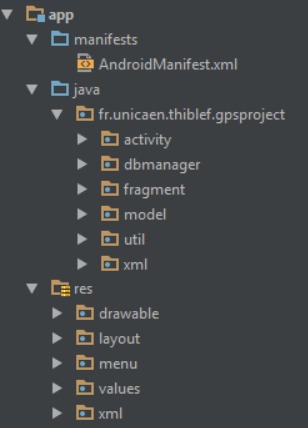
\includegraphics[scale=0.5]{img/archi.png}
  \caption{Architecture de l'application}
\end{img}

\begin{itemize}
  \item app
     \begin{itemize}
       \item manifests
       \begin{itemize}
         \item AndroidManifest.xml
       \end{itemize}
       \item java
       \begin{itemize}
         \item fr.unicaen.varlef.gpsproject
         \begin{itemize}
           \item activity
           \item dbmanager
           \item fragment
           \item model
           \item util
           \item xml
         \end{itemize}
       \end{itemize}
       \item res
       \begin{itemize}
           \item drawable
           \item layout
           \item menu
           \item values
           \item xml
         \end{itemize}
     \end{itemize}
\end{itemize}\bigskip

\end{multicols}




